%%%%%%%%%%%%%%%%%%%%%%%%%%%%%%%%%%%%%%%%%
% Beamer Presentation
% LaTeX Template
% Version 1.0 (10/11/12)
%
% This template has been downloaded from:
% http://www.LaTeXTemplates.com
%
% License:
% CC BY-NC-SA 3.0 (http://creativecommons.org/licenses/by-nc-sa/3.0/)
%
%%%%%%%%%%%%%%%%%%%%%%%%%%%%%%%%%%%%%%%%%

%----------------------------------------------------------------------------------------
%	PACKAGES AND THEMES
%----------------------------------------------------------------------------------------

\documentclass{beamer}

\mode<presentation> {

% The Beamer class comes with a number of default slide themes
% which change the colors and layouts of slides. Below this is a list
% of all the themes, uncomment each in turn to see what they look like.

%\usetheme{default}
%\usetheme{AnnArbor}
%\usetheme{Antibes}
%\usetheme{Bergen}
%\usetheme{Berkeley}
%\usetheme{Berlin}
%\usetheme{Boadilla}
%\usetheme{CambridgeUS}
\usetheme{Copenhagen}
%\usetheme{Darmstadt}
%\usetheme{Dresden}
%\usetheme{Frankfurt}
%\usetheme{Goettingen}
%\usetheme{Hannover}
%\usetheme{Ilmenau}
%\usetheme{JuanLesPins}
%\usetheme{Luebeck}
%\usetheme{Madrid}
%\usetheme{Malmoe}
%\usetheme{Marburg}
%\usetheme{Montpellier}
%\usetheme{PaloAlto}
%\usetheme{Pittsburgh}
%\usetheme{Rochester}
%\usetheme{Singapore}
%\usetheme{Szeged}
%\usetheme{Warsaw}

% As well as themes, the Beamer class has a number of color themes
% for any slide theme. Uncomment each of these in turn to see how it
% changes the colors of your current slide theme.

%\usecolortheme{albatross}
%\usecolortheme{beaver}
%\usecolortheme{beetle}
%\usecolortheme{crane}
%\usecolortheme{dolphin}
%\usecolortheme{dove}
%\usecolortheme{fly}
%\usecolortheme{lily}
%\usecolortheme{orchid}
%\usecolortheme{rose}
%\usecolortheme{seagull}
%\usecolortheme{seahorse}
%\usecolortheme{whale}
%\usecolortheme{wolverine}

%\setbeamertemplate{footline} % To remove the footer line in all slides uncomment this line
%\setbeamertemplate{footline}[page number] % To replace the footer line in all slides with a simple slide count uncomment this line

%\setbeamertemplate{navigation symbols}{} % To remove the navigation symbols from the bottom of all slides uncomment this line
}

\usepackage{graphicx} % Allows including images
\usepackage{booktabs} % Allows the use of \toprule, \midrule and \bottomrule in tables

%----------------------------------------------------------------------------------------
%	TITLE PAGE
%----------------------------------------------------------------------------------------

\title[Workshop TCMP]{Fortran \& Numerical Computations} % The short title appears at the bottom of every slide, the full title is only on the title page

\author{Rasyid Sulaeman} % Your name
\institute[UCLA] % Your institution as it will appear on the bottom of every slide, may be shorthand to save space
{
University of Indonesia \\ % Your institution for the title page
\medskip
\textit{rasyid.sulaeman@ui.ac.id} % Your email address
}
\date{\today} % Date, can be changed to a custom date

\begin{document}

\begin{frame}
\titlepage % Print the title page as the first slide
\end{frame}

\begin{frame}
\frametitle{Overview} % Table of contents slide, comment this block out to remove it
\tableofcontents % Throughout your presentation, if you choose to use \section{} and \subsection{} commands, these will automatically be printed on this slide as an overview of your presentation
\end{frame}

%----------------------------------------------------------------------------------------
%	PRESENTATION SLIDES
%----------------------------------------------------------------------------------------

%------------------------------------------------
\section{Introduction to Fortran} 
\subsection{Getting a feel for fortran}
\begin{frame}
\frametitle{What is Fortran?}

\begin{figure}
\centering
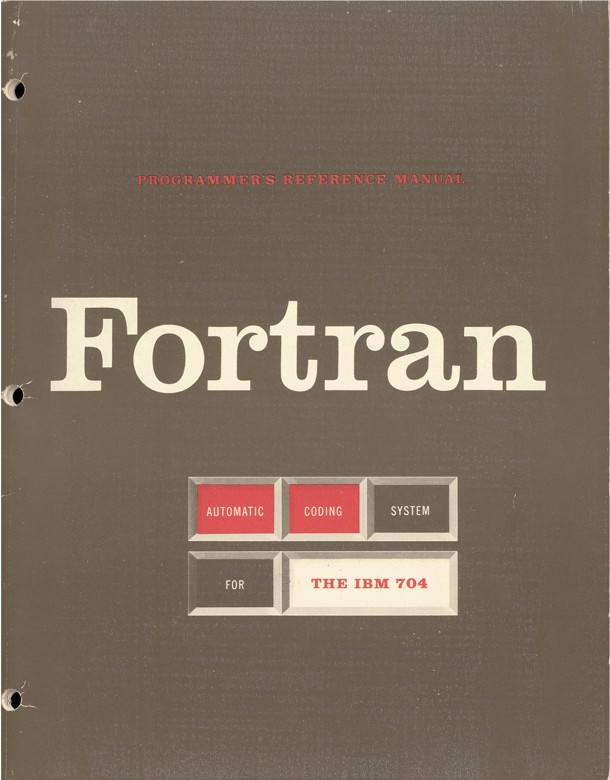
\includegraphics[scale=0.25]{Fortran_acs_cover.jpeg}
\end{figure}

\end{frame}

%------------------------------------------------

\begin{frame}
\frametitle{What is Fortran?}
\begin{itemize}
\item Programming language that is extensively used in numerical and scientific computing. 
\item Differ from other languages, Fortran have to be \textit{compiled} before run it on a computer.  
\end{itemize}
\end{frame}

%------------------------------------------------

\begin{frame}
\frametitle{Getting a Feel for Fortran}
\begin{figure}
\centering
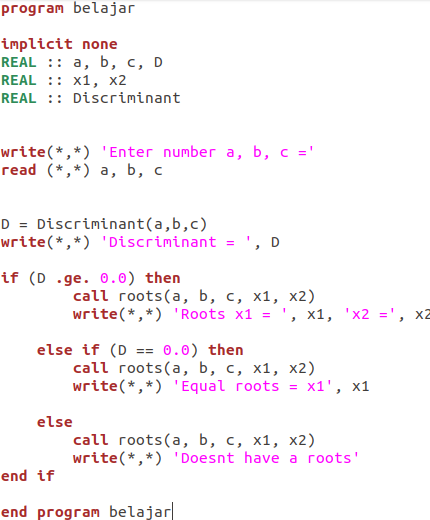
\includegraphics[scale=0.35]{tes.png}
\end{figure}
\end{frame}

%------------------------------------------------
\subsection{Let's get started}
\begin{frame}
\frametitle{Let's get started}
\begin{figure}
\centering

\includegraphics[scale=0.1]{letsgetstarted.jpg}
\end{figure}
\end{frame}

%------------------------------------------------
\section{Numerical Computation}
%------------------------------------------------
\subsection{Roots of Functions}
\begin{frame}
\frametitle{Roots of Functions}
\textbf{Bisection Method}
\begin{figure}
\centering
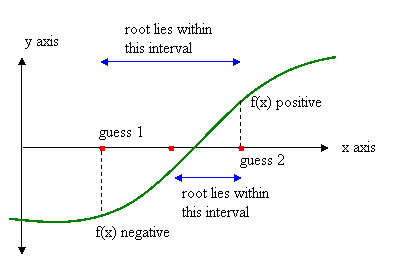
\includegraphics[scale=0.5]{Bisection.png}
\end{figure}
\end{frame}

%------------------------------------------------

\begin{frame}
\frametitle{Roots of Functions}
\textbf{Bisection Method}
\begin{block}{Principles}
Confine roots of a function in between two boundary, then \textbf{take a midpoint of the interval} continously in such a way we get a good approximation about the roots. 
\end{block}

\begin{itemize}
\item Guess the root of a functions
\item Determine the initial boundary that confine the root
\item Take a midpoint of the interval
\item Determine a region that have root
\item Repeat step 3 and 4 until \textbf{convegence}
\item You get your roots 
\end{itemize}
\end{frame}
%------------------------------------------------
\subsection{Solution of Linear System Equation}
\begin{frame}
\frametitle{Solution of Linear System Equation}
Linear system equations has a form:
\begin{equation}
\begin{matrix}
  a_{11}x_1 & +\; a_{12}x_2 & +\; a_{13}x_3 & \dots & +\; a_{1n}x_n \\
  a_{21}x_1 & +\; a_{22}x_2 & +\; a_{23}x_3 & \dots & +\; a_{2n}x_n \\
  a_{31}x_1 & +\; a_{32}x_2 & +\; a_{33}x_3 & \dots & +\; a_{3n}x_n \\
  \vdots & \vdots & \vdots & \ddots & \vdots \\
  a_{n1}x_1 & +\; a_{n2}x_2 & +\; a_{n3}x_3 & \dots & +\; a_{nn}x_n \\
 \end{matrix}
 \begin{matrix}
 \;=\;b_1 \\
 \;=\;b_2 \\
 \;=\;b_3 \\
 \;\vdots \\
 \;=\;b_n \\
 \end{matrix}
\end{equation}
\end{frame}

%------------------------------------------------
\begin{frame}
\frametitle{Solution of Linear System Equation}
\textbf{Gauss Elimination} \\
\begin{figure}
\centering
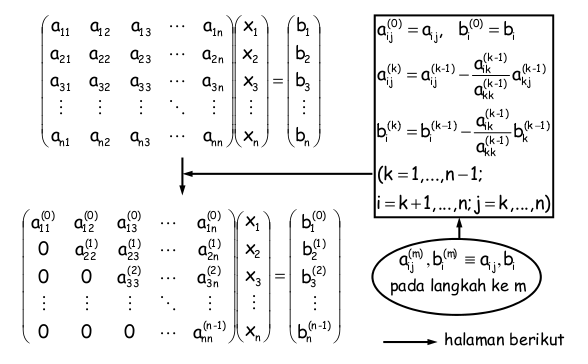
\includegraphics[scale=0.4]{sd.png}
\end{figure}
\end{frame}
%------------------------------------------------

\begin{frame}
\frametitle{Solution of Linear System Equation}
\textbf{Gauss Elimination}
\begin{figure}
\centering
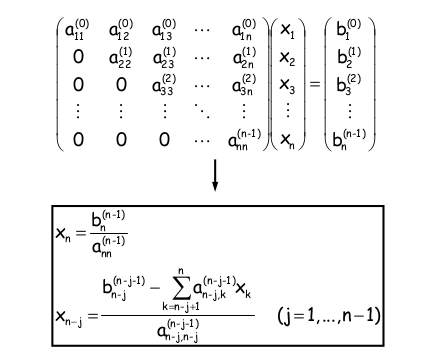
\includegraphics[scale=0.4]{cc.png}
\end{figure}
\end{frame}
%------------------------------------------------

\begin{frame}
\frametitle{Solution of Linear System Equation}
\textbf{Gauss Elimination} \\ 
So, Gauss elimination method consist of two steps:
\begin{itemize}
\item[1] Triangulation. Change matrix A into triangular matrix (so as matrix B)
\item[2] Do backwards substitution. Calculate $x$ by reverser order, from the last $x_n$ to $x_1$.
\end{itemize}
\end{frame}
%------------------------------------------------
\subsection{Numerical Differentiation}
\begin{frame}
\frametitle{Numerical Differentiation}
\textbf{Numerical Differentiation}
\begin{columns}[c]
\column{.45\textwidth}
\begin{figure}
\centering
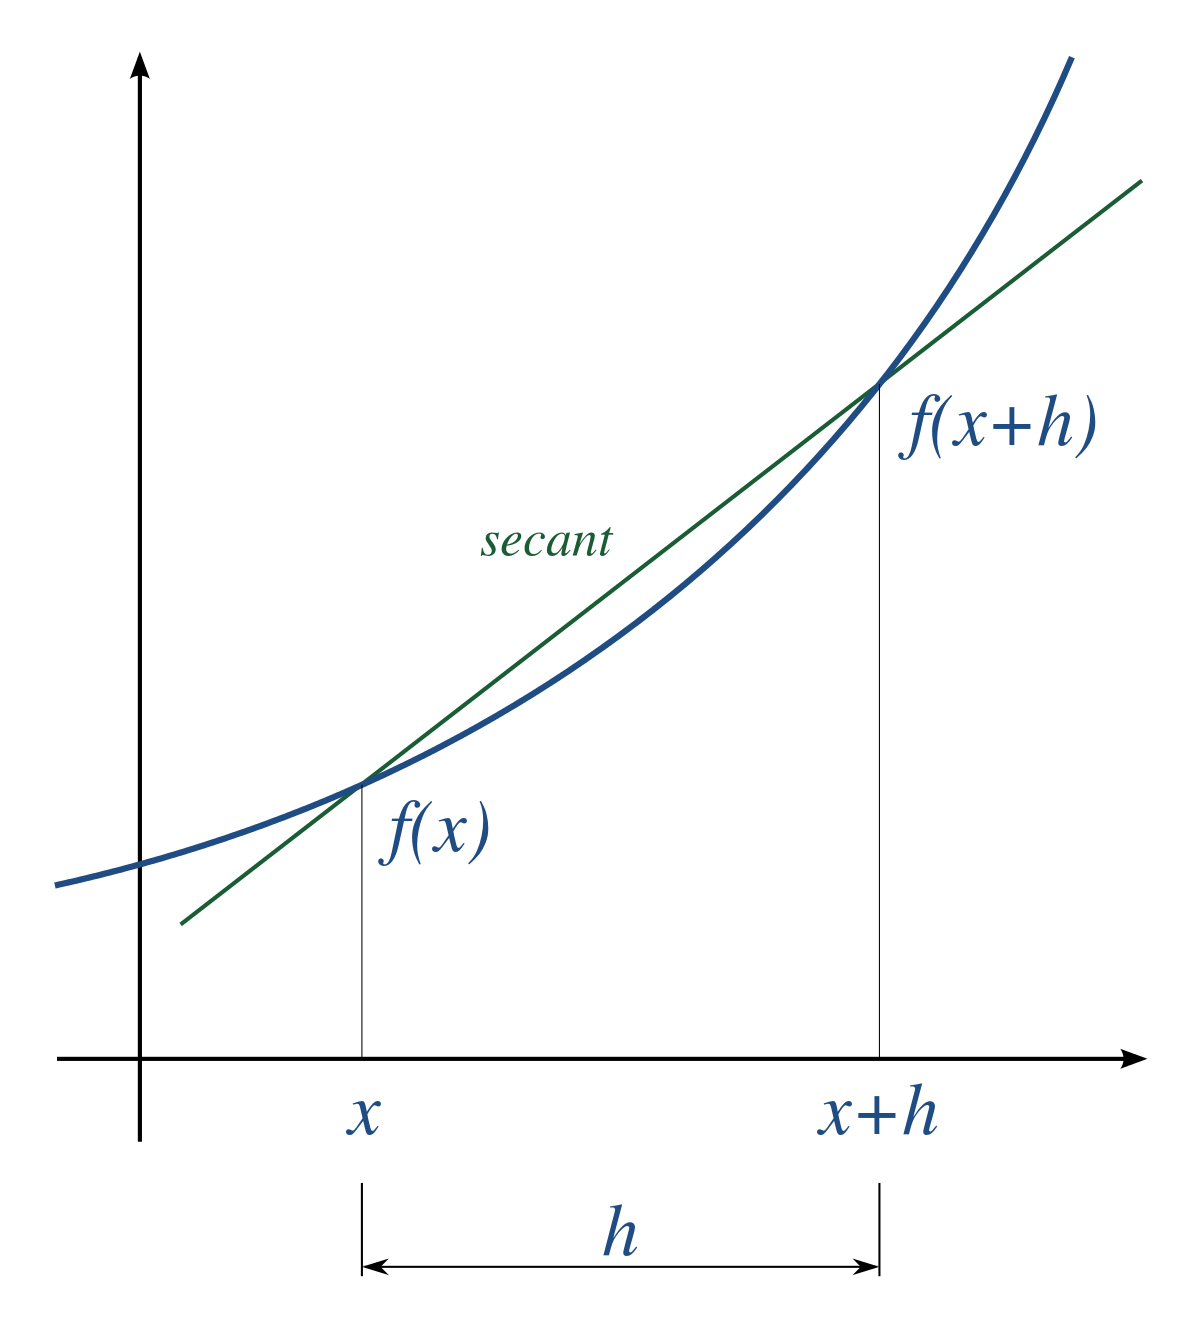
\includegraphics[scale=0.12]{diff.png}
\end{figure}
\column{.5\textwidth} 
A simple approximation of the first derivative is
\begin{equation*}
f^{\prime}(x) \approx \frac{f(x+h)-f(x)}{h}
\end{equation*}
\end{columns}


\end{frame}
%------------------------------------------------
\begin{frame}
\frametitle{Numerical Differentiation}
\textbf{Forward, Backward, and Central Finite Difference}
\begin{figure}
\centering
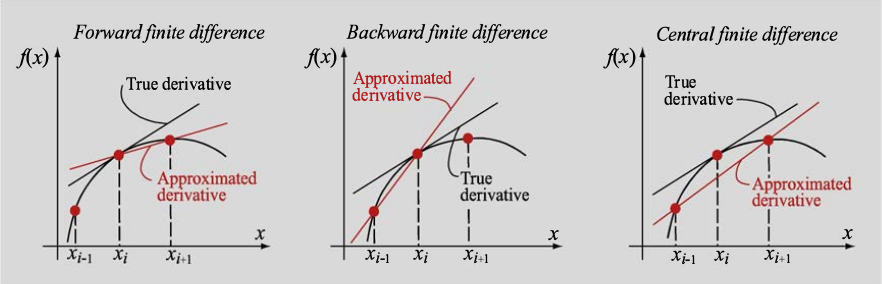
\includegraphics[scale=0.35]{fint.png}
\end{figure}
\end{frame}
%------------------------------------------------

\begin{frame}
\frametitle{Numerical Differentiation}
\textbf{Forward, Backward, and Central Finite Difference}
\begin{figure}
\centering
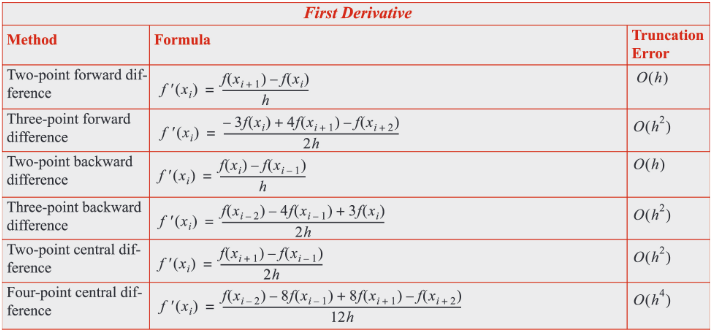
\includegraphics[scale=0.4]{table.png}
\end{figure}
\end{frame}
%------------------------------------------------
\begin{frame}
\Huge{\centerline{Terima Kasih}}
\end{frame}

%----------------------------------------------------------------------------------------

\end{document} 